\subsection{Introduction}

\begin{frame}
	\frametitle{What will we learn today ?}	
	\begin{itemize}
	\item {The distributed memory programming paradigm MPI}
	\item {Point-to-Point communications}
	\item {Collective communications}
	\item {Synchronizations}
	\end{itemize}
\end{frame}


\begin{frame}
	\frametitle{Reminder}
\begin{center}
%\includegraphics[width=8cm]{Day2/images/distributed.png}
%{\includegraphics[width=\textwidth]{Day2/images/distributed-memory.pdf}}
% Slide 41
\begin{tikzpicture}[node distance=8mm,
dots/.style={
  font=\sffamily,
  xshift=5mm,
  minimum width=1cm
},
node split/.append style = {xshift=5mm}
]

\tikzstyle{sample} = [-,thin]

  \node (node0)  [node split,]                  {$P_0$ \nodepart{second} $M_0$};
  \node (node1)  [node split,right of=node0]    {$P_1$ \nodepart{second} $M_1$};
  \node (dots)   [dots,right of=node1]          {$\ldots$};
  \node (nodeN)  [node split,right of=dots]     {$P_N$ \nodepart{second} $M_N$};
  \node (switch) [switch,below of=node1, xshift=6mm, yshift=-1cm]  {network or switch};

\path[sample] (node0.south) edge[out=-60,in=120] (switch.north);
\path[sample] (node1.south) edge[out=-60,in=120] (switch.north);
\path[sample] (nodeN.south) edge[out=-60,in=120] (switch.north);
\end{tikzpicture}

\end{center}
\end{frame}

\begin{frame}
\frametitle{Goals and scope of MPI}	
	\begin{itemize}
	\item {Provide a source-code portability}
	\item {efficiency across different architectures}
	\item {easier debugging}
	\item {parallel I/O}
	\end{itemize}
\end{frame}

\begin{frame}[containsverbatim]
\frametitle{MPI}
	\begin{itemize}
	\item {Run multiple instances of the same program : \verb+"mpirun -np p myApp myArgs"+ starts \verb+p+ instances of the program \verb+"myApp myArgs"+}
	\item {On the clusters : \verb+"srun -np p myApp myArgs"+}
	\item {Instances exchange information by sending messages to each other}
	\item {Communications take place within a \verb+communicator+ : a set of processes indexed from $0$ to $communicatorSize-1$. A special communicator named \verb+MPI_COMM_WORLD+ contains all the processes}
	\end{itemize}
\end{frame}


\begin{frame}[containsverbatim]
\frametitle{Hello World}

\begin{lstlisting}[language=C,frame=lines]
int main(int argc, char *argv[]){
   int size, rank;
   MPI_Init(&argc, &argv);
   MPI_Comm_size(MPI_COMM_WORLD, &size);
   MPI_Comm_rank(MPI_COMM_WORLD, &rank);

   printf("I'm process %d out of %d\n", rank, size);

   MPI_Finalize();
}
\end{lstlisting}
\begin{itemize}
	\item{Compile with \verb+mpicc hello.c -o hello+}
	\item{Run with \verb+srun -np 4 ./hello+}
\end{itemize}
\end{frame}


\subsection{One-to-One communications}

\begin{frame}[containsverbatim]
\frametitle{Types of communications in MPI}
	\begin{itemize}
	\item {Point-to-Point (One-to-One)}
	\item {Collectives (One-to-All, All-to-One, All-to-All)}
	\item {One-sided (One-to...)}
	\item {Blocking and Non-Blocking of all types}
	\end{itemize}
\end{frame}


\begin{frame}[containsverbatim]
\frametitle{MPI\_Send() and MPI\_Recv()}
	\begin{itemize}
	\item {\verb+MPI_Send(buf, count, datatype, destination, +\\ \verb+ tag, communicator)+}
	\item {\verb+MPI_Recv(buf, count, datatype, source, + \\ \verb+ tag, communicator, status)+}
	\item {Sends (receives) \verb+count+ elements of type \verb+datatype+ to (from) \verb+destination+ (\verb+source+) buffer \verb+buf+.}
	\item {{\bf Each send must be matched by a receive!}
		\begin{itemize}
			\item{You must know \verb+source+, \verb+tag+, \verb+communicator+ and size (\verb+count+ * \verb+sizeof(datatype)+) of incoming message}
			\item{If you don’t know, use \verb+MPI_Probe+ / \verb+MPI_Iprobe+ to get that information}
		\end{itemize}
	}
	\end{itemize}
	\textcolor{red}{Mismatches cause race conditions or deadlocks}
\end{frame}


\begin{frame}[containsverbatim]
\frametitle{ping.c}
\begin{lstlisting}[language=C,frame=lines]
int main(int argc, char *argv[]) {
   int rank, size;
   int buf[100];
   MPI_Status status;
   MPI_Init(&argc, &argv);
   MPI_Comm_rank(MPI_COMM_WORLD, &rank);
   MPI_Comm_size(MPI_COMM_WORLD, &size);
   if (rank == 0) {
      MPI_Send(buf, 100, MPI_INT, 1, 0, MPI_COMM_WORLD);
   } else {
      MPI_Recv(buf, 100, MPI_INT, 0, 0, MPI_COMM_WORLD,&status);
   }
   MPI_Finalize();
}
\end{lstlisting}

\end{frame}


\begin{frame}[containsverbatim]
\frametitle{watch out for deadlocks !}
\begin{itemize}
	\item{ping.c runs ok with 2 processes : \\
		\begin{tabular}{ c c c }
		  \underline{Process 0} &   & \underline{Process 1} \\
		  send(1,0) & $\longrightarrow$  & recv(0,0) \\
		  finalize() &  & finalize() \\
		\end{tabular}
	}
	\item{Deadlock if more than two processes : \\
		\begin{tabular}{ c c c c c}
		  \underline{Process 0} &   & \underline{Process 1} &  & \underline{Process 2} \\
		  send(1,0) & $\longrightarrow$  & recv(0,0) & & recv(0,0) \\
		  finalize() &  & finalize() \\
		\end{tabular}		
	}
\end{itemize}
\end{frame}


\begin{frame}[containsverbatim]
\frametitle{ping$\_$correct.c}
\begin{lstlisting}[language=C,frame=lines]
int main(int argc, char *argv[]) {
   int rank, size;
   int buf[100];
   MPI_Status status;
   MPI_Init(&argc, &argv);
   MPI_Comm_rank(MPI_COMM_WORLD, &rank);
   MPI_Comm_size(MPI_COMM_WORLD, &size);
   if (rank == 0) {
      MPI_Send(buf, 100, MPI_INT, 1, 0, MPI_COMM_WORLD);
   } else if (rank==1) {
      MPI_Recv(buf, 100, MPI_INT, 0, 0, MPI_COMM_WORLD,&status);
   }
   MPI_Finalize();
}
\end{lstlisting}
\end{frame}

\begin{frame}[containsverbatim]
\frametitle{Blocking point-to-point communications}
	\begin{itemize}
	\item {\verb+MPI_Send+ : Returns when buffer can be reused}
	\item {\verb+MPI_Bsend+ : (B for Buffer) : copy data in a local buffer and returns immediately }
	\item {\verb+MPI_Ssend+ : (S for Synchronous) : returns when other end posted matching recv}
	\item {\verb+MPI_Rsend+ : (R for Ready) : succeed only if the matching recv has been already posted}
	\item {\verb+MPI_Recv+ : Returns when message has been received }
	\item {\verb+MPI_Sendrecv+ : Sends and receive within the same call to avoid deadlocks}
	\item {\verb+MPI_Sendrecv_replace+ : sends, receive and replace buffer values using only one buffer}
	\end{itemize}
\end{frame}



\begin{frame}[containsverbatim]
\frametitle{Non-Blocking point-to-point communications}
	\begin{itemize}
	\item {\verb+MPI_Isend+ and \verb+MPI_Irecv+ : Do not wait for message to be buffered send/recv. Fills an additional \verb+MPI_Request+ parameter that identifies the request}
	\item {Do not use / modify / delete buffers until request completed}
	\item {Wait calls block until request(s) completed : 
		\begin{itemize}
			\item {\verb+MPI_Wait(request, status)+}
			\item {\verb+MPI_Waitall(count, array_of_requests,+\\ \verb+ array_of_statuses)+}
		\end{itemize}
	}
	\item {\verb+MPI_Issend+ : Non-blocking version of \verb+MPI_Ssend+}
	\item {\verb+MPI_Ibsend+ : Non-blocking version of \verb+MPI_Bsend+}
	\item {\verb+MPI_Irsend+ : Non-blocking version of \verb+MPI_Rsend+}
\end{itemize}
\end{frame}

%\begin{frame}[containsverbatim]
%\frametitle{MPI$\_$Request}
%
%An $MPI\_Request$ object has different purposes;
%
%\begin{itemize}
%	\item {The $MPI\_Send$ and $MPI\_Recv$ requests: internally identified as requests with specific types ($MPIR\_SEND$ and $MPIR\_RECV$}
%	\item {Persistent communication operations : they look like sends and receives, but are actually different from an implementation perspective}
%	\item {An $MPI\_Request$ is used to represent an operation, such as a nonblocking send, at several different stages of completion.  The state of the operation is encoded within the request}
%	\item {}
%\end{itemize}
%\end{frame}



\begin{frame}[containsverbatim]
\frametitle{Non-Blocking point-to-point communications (cont'd)}

Playing with \verb+MPI_Request+

\begin{itemize}
	\item {\verb+MPI_Waitsome+ : Waits for an MPI request to complete }
	\item {\verb+MPI_Waitany+ : Waits for any specified MPI Request to complete }
	\item {\verb+MPI_Test+ : Tests for the completion of a request }
	\item {\verb+MPI_Testall+ : Tests for the completion of all previously initiated requests }
	\item {\verb+MPI_Testany+ : Tests for completion of any previously initiated requests }
	\item {\verb+MPI_Testsome+ : Tests for some given requests to complete }
\end{itemize}
\end{frame}


\begin{frame}[containsverbatim]
\frametitle{iping.c}
\begin{lstlisting}[language=C,frame=lines]
int main(int argc, char *argv[]) {
   int rank;
   int buf[100];
   MPI_Request request;
   MPI_Status status;
   MPI_Init(&argc, &argv);
   MPI_Comm_rank(MPI_COMM_WORLD, &rank);
   if (rank == 0)
      MPI_Isend(buf, 100, MPI_INT, 1, 0,MPI_COMM_WORLD, &request);
   else if (rank == 1)
      MPI_Irecv(buf, 100, MPI_INT, 0, 0,MPI_COMM_WORLD, &request);
   MPI_Wait(&request, &status);
   MPI_Finalize();
}
\end{lstlisting}
\end{frame}


\begin{frame}[containsverbatim]
\frametitle{exchange.c}
Process 0 and 1 exchange the content of their buffer with non-blocking \label{call}
\begin{lstlisting}[language=C,frame=lines]
if (rank == 0) {
   MPI_Isend(buf1, 10, MPI_INT, 1, 0, MPI_COMM_WORLD, &request);
   MPI_Recv(buf2, 10, MPI_INT, 1, 0, MPI_COMM_WORLD, MPI_STATUS_IGNORE);
}else if (rank == 1){
   MPI_Isend(buf1, 10, MPI_INT, 0, 0, MPI_COMM_WORLD, &request);
   MPI_Recv(buf2, 10, MPI_INT, 0, 0,MPI_COMM_WORLD, MPI_STATUS_IGNORE);
}

MPI_Wait(&request, &status);
memcpy(buf1, buf2, 10*sizeof(int));
\end{lstlisting}
\end{frame}


\begin{frame}[containsverbatim]
\frametitle{exchange$\_$sendrecv.c}
Process 0 and 1 exchange the content of their buffer with sendrecv()
\begin{lstlisting}[language=C,frame=lines]
if (rank == 0)	{
   MPI_Sendrecv(buf1, 10, MPI_INT, 1, 0, buf2, 10, MPI_INT, 1, 0, MPI_COMM_WORLD, MPI_STATUS_IGNORE);
} else if (rank == 1) {
   MPI_Sendrecv(buf1, 10, MPI_INT, 0, 0, buf2, 10, MPI_INT, 0, 0, MPI_COMM_WORLD, MPI_STATUS_IGNORE);
}

memcpy(buf1, buf2, 10*sizeof(int));
\end{lstlisting}
\end{frame}

\begin{frame}[containsverbatim]
\frametitle{exchange$\_$sendrecv$\_$replace.c}
Process 0 and 1 exchange the content of their buffer with sendrecv$\_$replace()
\begin{lstlisting}[language=C,frame=lines]
if (rank == 0){
   MPI_Sendrecv_replace(buf1, 10, MPI_INT, 1, 0, 1, 0, MPI_COMM_WORLD, MPI_STATUS_IGNORE);
} else if (rank == 1) {
   MPI_Sendrecv_replace(buf1, 10, MPI_INT, 0, 0, 0, 0, MPI_COMM_WORLD, MPI_STATUS_IGNORE);
}
\end{lstlisting}
\end{frame}


\begin{frame}[containsverbatim]
\frametitle{Wildcard receives}
MPI$\_$ANY$\_$SOURCE and MPI$\_$ANY$\_$TAG are wildcards :
\begin{lstlisting}[language=C,frame=lines]
switch(rank) {
   case 0: MPI_Send(..., 1, 0, ...); break;
   case 1:
      MPI_Recv(..., MPI_ANY_SOURCE, MPI_ANY_TAG, ...);
      MPI_Recv(..., MPI_ANY_SOURCE, MPI_ANY_TAG, ...);
      break;
   case 2: MPI_Send(..., 1, 1, ...); break;
}
\end{lstlisting}
leads to : \\

\begin{tabular}{ c c c c c}
\underline{Process 0} &   & \underline{Process 1} &  & \underline{Process 2} \\
send(1,0) & $\longrightarrow$  & recv(*,*) & $\longleftarrow$ & send(1,1) \\
          & $\searrow$         & recv(*,*) & $\swarrow$       &           \\
\end{tabular}		
\end{frame}


\begin{frame}[containsverbatim]
\frametitle{MPI$\_$Barrier(communicator)}
Returns when all processes in communicator have joined
\begin{lstlisting}[language=C,frame=lines]
switch(rank) {
   case 0:
      MPI_Send(..., dest = 1, tag = 0, ...);
      MPI_Barrier(MPI_COMM_WORLD);  break;
   case 1:
      MPI_Recv(..., MPI_ANY_SOURCE, MPI_ANY_TAG, ...);
      MPI_Barrier(MPI_COMM_WORLD);
      MPI_Recv(..., MPI_ANY_SOURCE, MPI_ANY_TAG, ...);  break;
   case 2:
      MPI_Barrier(MPI_COMM_WORLD);
      MPI_Send(..., src = 1, tag = 1, ...);  break;
}\end{lstlisting}
\end{frame}

\begin{frame}[containsverbatim]
\frametitle{MPI$\_$Barrier(communicator) (cont'd)}
MPI$\_$ANY$\_$SOURCE and MPI$\_$ANY$\_$TAG are wildcards :

\begin{tabular}{ c c c c c}
\underline{Process 0} &   & \underline{Process 1} &  & \underline{Process 2} \\
send(1,0) & $\longrightarrow$  & recv(*,*) &  &  \\
\hline
{\bf barrier} &   & {\bf barrier} &  & {\bf barrier} \\
\hline
          &  & recv(*,*) & $\longleftarrow$       & send(1,1)   \\
\end{tabular}		

Order of calls on process 1 is important

\begin{itemize}
	\item{recv -- barrier -- recv \textcolor{green}{correct}}
	\item{barrier -- recv -- recv \textcolor{orange}{message race or deadlock (depends on msg size)}}
	\item{recv -- recv -- barrier \textcolor{red}{deadlock}}
\end{itemize}
\end{frame}


\begin{frame}[containsverbatim]
\frametitle{\textcolor{orange}{barrier -- recv -- recv}}

\begin{tabular}{ c c c c c}
\underline{Process 0} &   & \underline{Process 1} &  & \underline{Process 2} \\
send(1,0) & $\longrightarrow$  &  &  &  \\
 & $\searrow$  &  &  &  \\
\hline
{\bf barrier} &   & {\bf barrier} &  & {\bf barrier} \\
\hline
          &  & recv(*,*) & $\longleftarrow$       & send(1,1)   \\
          &  & recv(*,*) & $\swarrow$       &    \\
\end{tabular}		

Order of calls on process 1 is important

\begin{itemize}
	\item{recv -- barrier -- recv \textcolor{green}{correct}}
	\item{barrier -- recv -- recv \textcolor{orange}{message race or deadlock (depends on msg size)}}
	\item{recv -- recv -- barrier \textcolor{red}{deadlock}}
\end{itemize}
\end{frame}

\begin{frame}[containsverbatim]
\frametitle{\textcolor{red}{recv -- recv -- barrier}}

\begin{tabular}{ c c c c c}
\underline{Process 0} &   & \underline{Process 1} &  & \underline{Process 2} \\
send(1,0) & $\longrightarrow$  &  &  &  \\
          &  & recv(*,0) &    &   \\
          &  & recv(2,*) &      &    \\
\hline
{\bf barrier} &   & \textcolor{red}{{\bf barrier}} &  & {\bf barrier} \\
\hline
 &   &  & $\longleftarrow$ & \textcolor{red}{send(1,1)} \\
\end{tabular}		

Process 1 never enters the barrier since its second recv is never matched
\end{frame}


\subsection{Collective communications}


\begin{frame}[containsverbatim]
\frametitle{Collective communications}

\begin{center}
% Slide 152
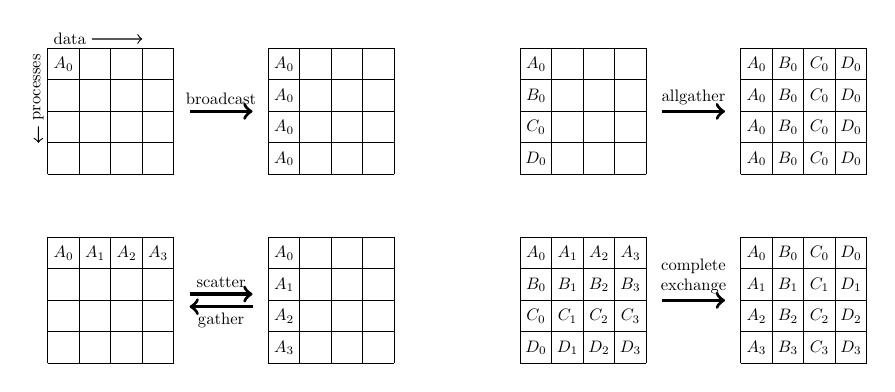
\begin{tikzpicture}[scale = 0.4, every node/.style={scale=0.6}]

\begin{scope}
	\begin{scope}
	\node[anchor = west] (Data) at (0, 4.3) {data};
	\node[anchor = east, rotate = 90] (Proc) at (-0.3, 4) {processes};
	\draw[->] (Data) -- (3, 4.3);
	\draw[->] (Proc) -- (-0.3, 1);
	\draw[step = 1cm] (0,0) grid (4,4);

	\node at (0.5, 3.5) {$A_0$};
	\end{scope}

	\draw[->, very thick] (4.5, 2) -- node[midway, above] {broadcast} (6.5, 2);

	\begin{scope}[xshift = 7cm]
	\draw[step = 1cm] (0,0) grid (4,4);

	\foreach \y in {0.5, 1.5, ..., 3.5}
		\node at (0.5, 4 - \y) {$A_0$};
	\end{scope}

	\begin{scope}[yshift = -6cm]
	\draw[step = 1cm] (0,0) grid (4,4);

	\foreach \x [count = \i from 0] in {0.5, 1.5, ..., 3.5}
		\node at (\x, 3.5) {$A_\i$};
	\end{scope}

	\draw[->, very thick] (4.5, -3.8) -- node[midway, above] {scatter} (6.5, -3.8);
	\draw[<-, very thick] (4.5, -4.2) -- node[midway, below] {gather} (6.5, -4.2);

	\begin{scope}[yshift = -6cm, xshift = 7cm]
	\draw[step = 1cm] (0,0) grid (4,4);

	\foreach \x [count = \i from 0] in {0.5, 1.5, ..., 3.5}
		\node at (0.5, 4 - \x) {$A_\i$};
	\end{scope}
\end{scope}

\begin{scope}[xshift = 15cm]
	\begin{scope}[yshift = 0cm]
	\draw[step = 1cm] (0,0) grid (4,4);

	\foreach \y/\l in {0.5/A, 1.5/B, 2.5/C, 3.5/D}
		\node at (0.5, 4 - \y) {$\l_0$};
	\end{scope}

	\draw[->, very thick] (4.5, 2) -- node[midway, above] {allgather} (6.5, 2);

	\begin{scope}[yshift = 0cm, xshift = 7cm]
	\draw[step = 1cm] (0,0) grid (4,4);

	\foreach \y in {0.5, 1.5, ..., 3.5} {
		\foreach \x/\l in {0.5/A, 1.5/B, 2.5/C, 3.5/D} {
			\node at (\x, 4 - \y) {$\l_0$};
		}
	}
	\end{scope}

	\begin{scope}[yshift = -6cm]
	\draw[step = 1cm] (0,0) grid (4,4);

	\foreach \y/\l in {0.5/A, 1.5/B, 2.5/C, 3.5/D} {
		\foreach \x[count = \i from 0] in {0.5, 1.5, ..., 3.5} {
			\node at (\x, 4 - \y) {$\l_\i$};
		}
	}
	\end{scope}

	\draw[->, very thick] (4.5, -4) -- node[midway, above, align = center] {complete \\ exchange} (6.5, -4);

	\begin{scope}[yshift = -6cm, xshift = 7cm]
	\draw[step = 1cm] (0,0) grid (4,4);

	\foreach \x/\l in {0.5/A, 1.5/B, 2.5/C, 3.5/D} {
		\foreach \y[count = \i from 0] in {0.5, 1.5, ..., 3.5} {
			\node at (\x, 4 - \y) {$\l_\i$};
		}
	}
	\end{scope}
\end{scope}

\end{tikzpicture}

\end{center}

\end{frame}



\begin{frame}[containsverbatim]
\frametitle{Collective communications}

\begin{itemize}
	\item{\verb+MPI_Bcast+ : Sends the same data to every process}
	\item{\verb+MPI_Scatter+ : Sends pieces of a buffer to every process of the communicator}
	\item{\verb+MPI_Gather+ : Retrieves pieces of data from every process}
	\item{\verb+MPI_Allgather+ : All pieces retrieved by all processes}
	\item{\verb+MPI_Reduce+ : Performs a reduction operation (\verb+MPI_SUM+, ...) across all nodes. E.g. dot product on distributed vectors}
	\item{\verb+MPI_Allreduce+ : Result distributed to all processes }
	\item{\verb+MPI_Alltoall+ : Sends all data to all processes}
	\item{{\bf Every process of the communicator must participate}. Parameters must match. Mismatches cause race conditions or deadlocks}
\end{itemize}

\end{frame}


\begin{frame}[containsverbatim]
\frametitle{Receiving image parts in order}
\begin{lstlisting}[language=C,frame=lines]
/* Generate image parts */
...
/* Each process sends */
   MPI_Isend(imgPart, partSize, MPI_BYTE, 0, 0, MPI_COMM_WORLD, &request);

// Process 0 receives all parts into buf
if (rank == 0){
   char *buf = malloc(nProcs*partSize);
   for (int i=0; i<nProcs; i++){
      MPI_Recv(buf + i*partSize, partSize, MPI_BYTE, i, 0, MPI_COMM_WORLD, MPI_STATUS_IGNORE);
   }

MPI_Wait(&request, MPI_STATUS_IGNORE);
\end{lstlisting}
\end{frame}


\begin{frame}[containsverbatim]
\frametitle{Receiving image parts out-of-order}
\begin{lstlisting}[language=C,frame=lines]
/* Generate image parts */
...
/* Each process sends */
   MPI_Isend(imgPart, partSize, MPI_BYTE, 0, 0, MPI_COMM_WORLD, &request);
// Process 0 receives all parts into buf
if (rank == 0) {
   char *buf = malloc(nProcs*partSize);
   MPI_Status s; int count;
   for (int i=0; i<nProcs; i++) {
      MPI_Probe(MPI_ANY_SOURCE, MPI_ANY_TAG, comm, &s);
      MPI_Get_count(&s, MPI_BYTE, &count);
      MPI_Recv(buf + s.MPI_SOURCE*count, count, MPI_BYTE, s.MPI_SOURCE, s.MPI_TAG, MPI_COMM_WORLD, MPI_STATUS_IGNORE);
} } MPI_Wait(&request, MPI_STATUS_IGNORE);
\end{lstlisting}
\end{frame}

\begin{frame}[containsverbatim]
\frametitle{Receiving image parts with a collective}
\begin{lstlisting}[language=C,frame=lines]
/* Generate image parts */
...
/* Process 0 is the root of the collective, i.e. the receiver of all parts */
int root = 0;
char *buf = NULL;
if (rank == root) /* Only the root must allocate buf */
   buf = malloc(nProcs*partSize)

   MPI_Gather(part, partSize, MPI_BYTE, buf, partSize, MPI_BYTE,  root, MPI_COMM_WORLD);
\end{lstlisting}
\end{frame}




\begin{frame}[containsverbatim]
\frametitle{Collectives within conditions}

Avoid collective calls within conditional clauses. What happens if :

\begin{lstlisting}[language=C,frame=lines]
int root = 0;
char *buf = NULL;
if (rank == root) { /* Only the root must allocate buf */
   buf = malloc(nProcs*partSize)

   MPI_Gather(part, partSize, MPI_BYTE, buf, partSize, MPI_BYTE,  root, MPI_COMM_WORLD);
}else{
   MPI_Send(part, ... , ... , rank, MPI_TAG);
}
\end{lstlisting}
\end{frame}


\subsection{Customization}


\begin{frame}[containsverbatim]
\frametitle{Customized communicators and datatypes}

\begin{itemize}
	\item{ You can define your own communicators : 
	\begin{itemize}
		\item{\verb+MPI_Comm_dup+ duplicates a communicator (e.g. to enable private communications within library functions)}
		\item{\verb+MPI_Comm_split+ splits a communicator into multiple smaller communicators (useful when using 2D and 3D domain decompositions) }
	\end{itemize}
	}
	\item{ You can define custom datatypes :
	\begin{itemize}
		\item{Simple structs (\verb+MPI_Type_struct+)}
		\item{Vectors (\verb+MPI_Type_vector+)}
		\item{{\bf NO POINTERS}}
	\end{itemize}
	}
\end{itemize}

\end{frame}

\subsection{Summary}

\begin{frame}[containsverbatim]
\frametitle{Does this program terminate? (assume 2 processes)}
\begin{lstlisting}[language=C,frame=lines]
int rank;
MPI_Init(&argc, &argv);
MPI_Comm_rank(&rank, MPI_COMM_WORLD);
if (rank)
  MPI_Send(&rank, 1, MPI_INT, 0, 0, MPI_COMM_WORLD);
else
  MPI_Recv(&rank, 1, MPI_INT, 1, 0, MPI_COMM_WORLD, MPI_STATUS_IGNORE);

if (rank)
  MPI_Send(&rank, 1, MPI_INT, 0, 0, MPI_COMM_WORLD);
else
  MPI_Recv(&rank, 1, MPI_INT, 1, 0, MPI_COMM_WORLD, MPI_STATUS_IGNORE);

MPI_Finalize();
\end{lstlisting}
\end{frame}

\begin{frame}[containsverbatim]
\frametitle{Timing MPI programs}

\begin{itemize}
	\item {\verb+MPI_Wtime()+ : returns a double precision floating point number, the time in seconds since some abritrary point of time in the past }
	\item {\verb+MPI_Wtick()+ : returns a double precision floating point number, the time in seconds between successive ticks of the clock }
	\item { both functions are not synchronized across the running processors. }
\end{itemize}
\end{frame}


\begin{frame}[containsverbatim]
\frametitle{Next time}

That's all for MPI 1.0. What's new in MPI2 :

\begin{itemize}
	\item {Parallel I/O}
	\item {One-sided communications}
	\item {Dynamic process management}
\end{itemize}

\end{frame}


\begin{frame}
\frametitle{Implementation of MPI}	
You don't need to have always access to a cluster or a supercomputer to develop parallel applications. Here follows some implementations of MPI :
	\begin{itemize}
	\item {\textbf{Linux} OpenMPI, MPICH2, IntelMPI (licensed)}
	\item {\textbf{MacOS X} OpenMPI (without Fortran for the official port, with if installing by hand), MPICH2 (via homebrew)}
	\item {\textbf{Windows} OpenMPI, MPICH1 (older version), MS-MPI }
	\end{itemize}
\end{frame}



%%% Local Variables: 
%%% mode: latex
%%% TeX-master: "../cours_vince"
%%% End: 
